\documentclass{beamer}
\usetheme{fdu}

%%% Packages
\usepackage{tikz} % plot in place
\usepackage{pgfplots} % rather include jpg/pdf
\pgfplotsset{compat=1.9}
\usepackage{diagbox} % diagbox for table
\usepackage[export]{adjustbox} % autofix for table
\usepackage[ruled]{algorithm2e}
\SetAlCapFnt{\tiny\sffamily} % setting fonts for algorithm caption
\usepackage[round]{natbib} % bib cite package
\bibliographystyle{dinat} % set bib style
\setbeamercovered{transparent} % shadow words for overlay
\usepackage{listings}
\usepackage{xeCJK} % CJK package for xelatex
\setCJKmainfont{SimHei} % use SimHei as main font <- need preinstall SimHei
%\setbeamertemplate{caption}[numbered] % add caption number for figure and table

%%% Titlepage information
\title[Short Title]{Long Title Here}
\author[Presenter Name]{\textbf{Presenter Name} \and Author2 \and Author3}
\institute[Fudan University]{
    School of Computer Science, Fudan University, Shanghai, China \\
    Shanghai Key Laboratory of Data Science, Shanghai, China \\
    Shanghai Institute of Intelligent Electronics \& Systems \\~\\
    % Thanks funding here
    \tiny{This work is partially supported by xxx}
}

% table of contents
\AtBeginSection[]{
    \begin{frame}<beamer>{Agenda}
    \tableofcontents[
        currentsection,
        currentsubsection, 
        hideothersubsections, 
        sectionstyle=show/shaded,
    ]
    \end{frame}
}

\begin{document}

\begin{frame}
  \titlepage
\end{frame}

\section{SectionName}
\begin{frame}{Frame title here (optional)}{Frame subtitle here (also optional)}
  whatever you want to say\\
  中文支持ok
\end{frame}

\section{Examples}
\subsection{itemize}
\begin{frame}[t]{itemize}
  The main contribution of our work is to propose a xxxx
  \begin{itemize}
    \item point one
          \begin{itemize}
            \item \textbf{Point1.1}
            \item something about point 1
            \item \textbf{Point1.2}
            \item something about point 2
            \item \textbf{Point1.3}
            \item something about point 3
          \end{itemize}
    \item point two
    \item point three
    \item point four
  \end{itemize}
\end{frame}

\subsection{enumerate}
\begin{frame}[t]{enumerate}
  \begin{enumerate}
    \item First,
    \item Second,
  \end{enumerate}
\end{frame}

\subsection{columns}
\begin{frame}{columns}
  \begin{columns}
    \begin{column}{.7\textwidth}
      0.7 textwidth
      
\includegraphics[width=\textwidth]{resources/placeholder1}
    \end{column}

    \begin{column}{.3\textwidth}
      0.3 textwidth
      
\includegraphics[width=\textwidth]{resources/placeholder1}
    \end{column}
  \end{columns}
\end{frame}

\subsection{images}
\begin{frame}[t]{images}
  \centering
  
\includegraphics[width=\textwidth]{resources/placeholder1}
\end{frame}

\subsection{animation}
\begin{frame}{}
  \begin{columns}
    \begin{column}{.5\textwidth}
      \begin{itemize}
        \item<1-> \textbf{Point1}
        \item<1> \scriptsize{something about point 1}
        \item<2-> \textbf{Point2}
        \item<2> \scriptsize{something about point 2}
        \item<3-> \textbf{Point3}
        \item<3> \scriptsize{something about point 3}
      \end{itemize}
    \end{column}

    \begin{column}{.5\textwidth}
      \begin{onlyenv}<1-3>
        \begin{center}
          \includegraphics<1>[width=\textwidth]{resources/placeholder1}%
          \includegraphics<2>[width=\textwidth]{resources/placeholder2}%
          \includegraphics<3>[width=\textwidth]{resources/placeholder3}%
        \end{center}
      \end{onlyenv}
    \end{column}
  \end{columns}
\end{frame}

\subsection{cite}
\begin{frame}[t]{cite}
  \begin{itemize}
    \item First you need to put all your reference into the bib file like reference.bib
    \item Then you can cite like this Author (year) -> \cite{jia2014caffe}
    \item footnote cite seems not good...If you find better way to call footnote, please issue for me.
    \item footnote \footnote{\citep*{jia2014caffe}}
  \end{itemize}
\end{frame}

\subsection{block}
\begin{frame}{block}
  \begin{block}{Block Title}
    Anything you want to emphasize
  \end{block}
\end{frame}

\subsection{equation}
\begin{frame}{equation}
  \begin{equation}
    \Sigma + \epsilon + \alpha + \beta + \Theta
  \end{equation}
\end{frame}

\subsection{algorithm}
\begin{frame}{algorithm}
  \begin{columns}
    \begin{column}{0.5\textwidth}
      \begin{algorithm}[H]
        \LinesNumbered
        \caption{\tiny{Algorithm Title}}
        \label{alg:A}
        \tiny
        \KwIn{\\
          ~~Variables one, $one$ \\
          ~~Variables two, $two$ \\
        }
        \KwOut{\\
          ~~Output, $out$ \\
        }
        \ForEach{condition}{
          loop
        }
        \If{condition}{
          process
        }
        \eIf{condition}{
          process
        }{
          else process
        }
      \end{algorithm}
    \end{column}

    \begin{column}{0.5\textwidth}
      \begin{itemize}
        \item Detail for your algorithm
      \end{itemize}
    \end{column}
  \end{columns}
\end{frame}

\subsection{code}
\begin{frame}[fragile]{source code}
  \lstinputlisting[language=C,caption=C code example]{resources/hello.c}
  you should pass the option fragile to the frame environment.
\end{frame}

\subsection{tikz}
\begin{frame}{tikz plot inplace}
  \begin{figure}
    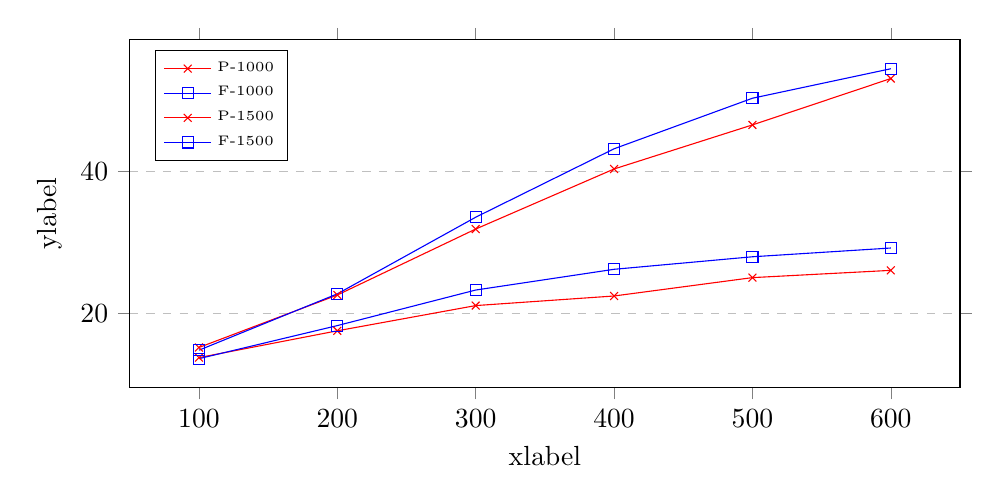
\begin{tikzpicture}
      \begin{axis}[
          width=\textwidth,
          height=6cm,
          xlabel={xlabel},
          ylabel={ylabel},
          ymajorgrids=true,
          tick align=outside,
          legend pos=north west,
          grid style=dashed,
        ]

        \addplot[draw=red,mark=x] coordinates {
            (100,13.7755) (200,17.5504) (300,21.1028) (400,22.4519) (500,25.0381) (600,26.0604)
          };
        \addlegendentry{\tiny{P-1000}}

        \addplot[draw=blue,mark=square] coordinates {
            (100,13.6265) (200,18.2843) (300,23.2898) (400,26.2097) (500,27.9736) (600,29.2072)
          };
        \addlegendentry{\tiny{F-1000}}

        \addplot[draw=red,mark=x] coordinates {
            (100,15.2016) (200,22.5882) (300,31.8770) (400,40.3320) (500,46.5383) (600,53.0686)
          };
        \addlegendentry{\tiny{P-1500}}

        \addplot[draw=blue,mark=square] coordinates {
            (100,14.8190) (200,22.7503) (300,33.5406) (400,43.1775) (500,50.2947) (600,54.4454)
          };
        \addlegendentry{\tiny{F-1500}}
      \end{axis}
    \end{tikzpicture}
    \caption{place some explanation here}
  \end{figure}
\end{frame}

\section{Q\&A}
\begin{frame}{Thanks Q\&A}
  \titlepage
\end{frame}

\begin{frame}[t]{References}
  \tiny
  \bibliography{reference}
\end{frame}

\end{document}
